\documentclass{article}

\usepackage[utf8]{inputenc}
\usepackage[ngerman]{babel}
\usepackage{amssymb}
\usepackage{amsmath}
\usepackage{graphics}
\usepackage{stmaryrd}

% Pseudocode
\usepackage{algorithm}
\usepackage[noend]{algpseudocode}
\usepackage{graphicx}
\usepackage{pdfpages}

\usepackage{tikz}

\setlength{\parindent}{0in}

\newcommand{\zettelNummer}{11}
\newcommand{\studierenderEins}{Eli Kogan-Wang (7251030)}
\newcommand{\studierenderZwei}{David Noah Stamm (7249709)}
\newcommand{\studierenderDrei}{Daniel Heins (7213874)}
\newcommand{\studierenderVier}{Tim Wolf (7269381)}

\newcounter{AufgabenCounter}
\setcounter{AufgabenCounter}{1}
\newcounter{TeilaufgabenCounter}
\newenvironment{aufgabe}{\section*{Aufgabe \theAufgabenCounter}\setcounter{TeilaufgabenCounter}{1}}{\stepcounter{AufgabenCounter}}
\newenvironment{teilaufgabe}{\paragraph*{\alph{TeilaufgabenCounter})}}{\stepcounter{TeilaufgabenCounter}}

\renewcommand{\to}{\textnormal{ to }}
\newcommand{\bigO}{\mathcal{O}}

\newcommand{\qed}{\hfill$\square$}

\begin{document}

\title{Datenstrukturen und Algorithmen \\ Heimübung \zettelNummer{}}
\author{\studierenderEins{} \\
  \studierenderZwei{} \\
  \studierenderDrei{} \\
  \studierenderVier{}}

\maketitle

% Aufgabe 1
\begin{aufgabe}
  Sei $G=(V,E)$ ein ungerichteter Graph.

  \textbf{Zu zeigen}: Nach DFS$(G,s)$ für ein $s\in V$ ist jede von $s$ erreichbare Kankte
  $e\in E_{\text{connected }s}$ eine Baumkante des DFS-Baums, eine Rückwärts/Vorwärtskante.

  \textbf{Beweis}:
  Sei $e\in E_{\text{connected }s}$ eine von $s$ erreichbare Kante.
  Das heißt, dass für $e={v_1,v_2}$ mit $v_1\neq v_2$, der Startknoten $v_1$ im DFS-Baum liegt,
  und da der Baum bzgl. der Zusammenhangskomponente von $s$ vollständig ist, auch
  $v_2$ im DFS-Baum liegt.

  Nun lässt sich eine Fallunterscheidung durchführen:

  Wenn $e$ im DFS-Baum liegt, dann ist $e$ eine Baumkante.

  Wenn $e$ nicht im DFS-Baum liegt, dann ist $e$ eine Rückwärts/Vorwärtskante.
  Da $e$ zwei Knoten aus dem DFS-Baum verbindet. Betrachtet man
  $e$ als gerichtet, so kann man betrachten, ob $v_1$ vor oder nach $v_2$ in der topologischen Sortierung
  des Baumes vorkommt.
\end{aufgabe}
\begin{aufgabe}

  Wir beginnen mit dem Ergebnis des Algorithmus Tran: $E^*$. $O(|V|^2 + |V|\cdot |E|)$

  In $O(|V|^2)$ reduzieren wir
  $E^*$ zu
  $E^{*\prime}=\{(u,v)|\text{Es existiert ein Weg in $G$ von $u$ nach $v$ und von $v$ nach $u$}\}$.

  Und reduzieren dann $E^{*\prime}$ zur ungerichteten unterliegenden Kantenmenge $E^{*\prime\prime}=\{\{u,v\}|\text{Es existiert ein Weg in $G$ von $u$ nach $v$ und von $v$ nach $u$}\}$ auch in $O(|V|^2)$.

  Nun führen wir Suchen (Tiefen oder Breitensuche) maximal $|V|$ mal in $G''=(V,E^{*\prime\prime})$ durch, um die einzelnen Zusammenhangskomponenten zu entfernen.

  $|V|$ mal, da es maximal $|V|$ Zusammenhangskomponenten (eine für jeden Knoten) gibt.

  Das geschieht in einer Laufzeit von $O((|V| + |E|)\cdot |V|)=O(|V|^2+|V|\cdot|E|)$.

  Der Algorithmus beruht auf der Korrektheit von Tran und extrahiert mithilfe von korrekten
  Suchen starke Zusammenhangskomponenten auf.
  Die Starken zusammenhangskomponenten bilden innerhalb der doppelt transitiven ungerichteten Hülle die regulären starken
  Zusammenhangskomponenten, die klassisch mit Suchen entdeckt werden können.
\end{aufgabe}

\begin{aufgabe}
  \begin{teilaufgabe}
    Der Algorithmus funktioniert wie zuvor.

    Sei $(u,v)$ eine Kante mit Gewichtung $0$.

    Nachdem $u$ aus dem Heap entfernt wurde und zur Menge $S$ der entdeckten Knoten
    hinzugefügt wurde, wird $d(v)$ auf $d(u)+0$ gesetzt und $v$
    darauffolgend entfernt (mit Knoten mit derselben Distanz).

    Damit wird $v$ Zeitlich richtig im Algorithmus entfernet.
  \end{teilaufgabe}
  \begin{teilaufgabe}
    Wir betrachten diesen Graphen:\\
    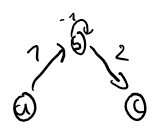
\includegraphics[scale=1]{2022-06-26-Blatt-11-3-b.png}

    Dijkstra von $a$ aus:

    \vspace{0.5cm}

    $S=\{a\}$

    \vspace{0.5cm}

    \begin{tabular}{l|l|l}
      $V\backslash S$ & b   & c        \\
      $d(a)$          & $1$ & $\infty$ \\
      $\pi(a)$        & $a$ & $\infty$
    \end{tabular}

    \vspace{1cm}

    $S=\{a,b\}$ $d(b)=1$

    \vspace{0.5cm}

    \begin{tabular}{l|l|}
      $V\backslash S$ & c   \\
      $d(a)$          & $2$ \\
      $\pi(a)$        & $b$
    \end{tabular}

    \vspace{1cm}

    Nach Dijkstra ist der kürzeste Weg: $a\rightarrow b\rightarrow c$ mit Gesamtlänge $3$.

    $\lightning$ kürzester Weg ist $a\rightarrow b\rightarrow b\dots b\rightarrow c$ mit Gesamtlänge $-\infty$.
  \end{teilaufgabe}
\end{aufgabe}

\end{document}
